\documentclass[a4paper,12pt]{report}
\renewcommand{\baselinestretch}{1.5}
\usepackage[margin=2.5cm, inner=4cm, outer=2cm]{geometry}
\usepackage[T1]{fontenc}
\usepackage[utf8]{inputenc}
\usepackage{lmodern}
\usepackage{graphicx}
\usepackage[german]{babel}

\title{Funktionsweise eines Raycasters mithilfe eines selber geschriebenen Beispiels erkl\"art}
\author{Andreas Gwilt}

\begin{document}

\maketitle
\tableofcontents

\begin{abstract}
This looks rather concrete to me. Actually, no it doesn't.
\end{abstract}

\section{Was ist ein Raycaster?}
% say roughly what it is, and what i'm trying to do in the FA
Raycasting ist ein ziemlich weiter Begriff, der meistens für eine Rendermethode benutzt wird. Allgemein ist es eine Technik, um zu sehen, ob ein Strahl eine Fläche schneidet. Man ``wirft'' einen Strahl, und überprüft, ob er eine Ebene schneidet oder nicht. Diese ist dem Raytracing sehr ähnlich, aber ist viel limitierter und auch schneller.
Ich habe, um den Raycaster zu erklären, eine in der ersten Person gerenderten Version von Conways \textit{Spiel des Lebens} geschrieben. 

\begin{figure}[htbp] 
        \centering
        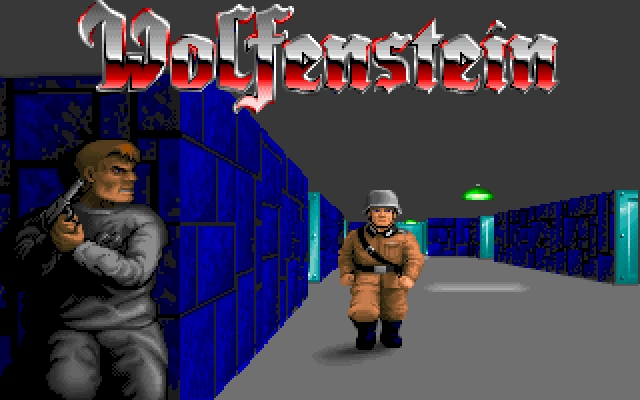
\includegraphics[width=4in]{wolfenstein-cover.jpg} 
        \caption{Wolfenstein 3D, ein Spiel, das einen Raycaster verwendete.}
\end{figure}

\subsection{Welche Probleme löst ein Raycaster?}
Raycasting ist eine Methode, um zu überprüfen, ob ein Strahl eine Fläche schneidet oder nicht. Die häufigste Anwendung dafür ist als einfaches Renderverfahren, um ein Spielfeld in Pseudo-3D darzustellen. Es gibt aber auch mehrere andere Anwendungen, z.B. Kollisionserkennung oder um fest zu stellen, ob etwas sichtbar ist oder nicht. In meinem Beispiel nutze ich die Methode (in der \texttt{cast()} Funktion) hauptsächlich dazu, das Spielfeld darzustellen, aber auch als Kollisionserkennung für die \texttt{walk()} Funktion. Ich werde mich jedoch auf den Raycaster als Rendermethode konzentrieren. Raycasting wird auch meistens in Spielen benutzt, wo schnelles Rendern wichtig ist, wodurch es als realistische Rendermethode nicht geeignet ist. \\
In den frühen 1990ern, als Raycasting beliebt wurde, hatte man noch ziemlich wenig Rechenleistung, wollte aber ``3D'' Spiele schreiben. Eine wirklich dreidimensionales Spiel-Engine (wie die 1996 erschienene Quake Engine) war noch nicht schnell genug, um in einem Spiel benutzt zu werden, also verwendete man Methoden wie Raycasting, um die Illusion von 3D herzustellen. Das vielleicht berühmteste Spiel, was Raycasting benutzte, war wahrscheinlich Wolfenstein 3D (Auch der erste beliebte Ego-Shooter). Wolfenstein 3D, auch Wolf3D genannt, hatte ein zweidimensionales Spielfeld, was in 3D dargestellt wurde. \\
Raycasting musste jedoch sehr viele Kompromisse eingehen, um so schnell zu sein. Das Spielfeld war ein zweidimensionales Array, also konnte es nur Rechte Winkel geben, und Decke und Boden mussten immer gleich hoch bleiben. Man erkennt an dem Screenshot von Wolf3D deutlich, dass das Spiel nicht wirklich dreidimensional ist. Auch sieht das Bild blockhaft aus, und die Beleuchtung ist nicht realistisch.

\subsection{Die Geschichte des Raycasters}
Raycasting wurde schon diskutiert, lange bevor PCs leistungsstark genug waren, um es wirklich in Spielen zu benutzen. Eine 1982 veröffentlichte Abhandlung von Scott Roth beschreibt Raycasting als Methode, dreidimensionale Körper zu rendern. \\
Eines der ersten Spiele, die das Prinzip implementierten, war \textit{Hovertank 3D}, was in April 1991 von id Software in einem Magazin veröffentlicht wurde. \textit{Hovertank 3D} war noch sehr primitiv und hatte noch keine Texturen auf den Wänden, noch dazu wurde es nicht für eine große Zielgruppe veröffentlicht, aber es war der Anfang eines neuen Genre von Spielen. Im darauffolgenden November erschien \textit{Catacomb 3-D}, was Texturen hatte, und oft als der erste Ego-Shooter gesehen wird. \\
Zufrieden mit den zwei ``Prototypen'' entwickelten id Software ihr neues Spiel \textit{Wolfenstein 3D}, das die Technologie von \textit{Catacomb 3-D} übernahm. \textit{Wolfenstein 3D}, was 1992 von Apogee Software veröffentlicht wurde, war ein großer Erfolg und machte Ego-Shooter, und damit den Raycaster, bekannt. Danach schaffte id Software das revolutionäre Spiel \textit{DOOM}. \textit{DOOM} war ein noch viel größerer Erfolg, der eine sehr verbesserten Spiel-Engine hatte. Die neue Engine war jedoch nicht mehr wirklich ein echter Raycaster, sondern benutzte Binary Space Partitioning und andere fortgeschrittene Methoden. Heutzutage findet der Raycaster nicht mehr viel Verwendung als Renderer, aber das Prinzip wird mit dem Raytracer fortgeführt. Der Raytracer arbeitet immer in drei Dimensionen, und ist rekursiv, d.h. er simuliert den kompletten Gang eines Lichtstrahles, inklusiv Reflexionen. Raytracing ist aber noch immer zu langsam für Echtzeit Darstellung, und findet eher als Renderer von stillen Bildern Gebrauch.

\section{Wie funktioniert ein Raycaster?}
\subsection{Allgemein}
\subsubsection{Daten}
Die Informationen (z.B. das Spielfeld oder die Spielerposition) müssen auf bestimmte Art gespeichert werden, um von dem Raycaster benutzt zu werden. In meiner Implementierung habe ich eine Funktion, die einen Strahl in einem bestimmten Winkel von einem bestimmten Punkt wirft: \texttt{cast(world, p\_x, p\_y, a)}. Die Welt wird als zweidimensionales Array gespeichert, in dessen Feldern 1 für eine Wand oder Zelle steht, und 0 für leeren Raum. Man könnte auch Farben speichern, oder mehrere Zahlen für mehrere Texturen/Farben haben. Meistens würde man nur Wände speichern, aber ich habe als Spiel Conways \textit{Spiel des Lebens} genommen, ein zweidimensionaler Zelluläre Automat, in dem das Spielfeld in dem eben beschriebenen Format gespeichert wird. Man kann aber zwischen einem Kartesischen Koordinatensystem, in dem (0,0) unten links ist, und einem Array Kartesischen Koordinatensystem, in dem (0,0) oben links ist, wählen. Ich habe mich für (0,0) unten links entschieden, da es (meiner Ansicht nach) leichter verständlich ist. \\
Dann muss man die Spielerposition speichern (die Variablen \texttt{p\_x} und \texttt{p\_y}). Diese Koordinaten sind aber in einem anderen Format als das Spielfeld. Man will nämlich den Spieler innerhalb eines Feldes bewegen können. Also hat man eine Konstante (\texttt{TILE}), die die Länge eines Feldes beschreibt. Um zu bestimmen, in welchem Feld der Spieler steht, rechnet man einfach \texttt{world[p\_x // TILE][p\_y // TILE]}: man teilt ohne Rest die Spielerkoordinaten durch die Feldlänge \texttt{TILE}. \\
Der Winkel des Spielers oder des Strahls ist auch wichtig. Da die Python-Funktionen für sin, cos, etc. das Bogenmaß annehmen, habe ich alle Winkel so gespeichert. Die Funktionen gehen auch davon aus, dass ein Winkel immer positiv und unter 2$\pi$ bleiben wird. Die "Richtung" der Winkel muss man auch selber definieren, aber ich habe 0 als rechts definiert, und $\pi$/2 als unten (auf die x-Achse zeigend).
\subsubsection{Was ist die Aufgabe des Raycasters?}
Here goes stuff explaining what things the RC needs to do in a program, as opposed to things like adding sprites, etc.

\subsection{Schritt für Schritt Erklärung}
Here goes a top-down explanation of how my code works (and obviously how the RC works).

\section{Zusammenfassung}
One or two paragraphs of TL;DR.

\end{document}
